% !TeX program = xelatex
\documentclass[11pt,a4paper]{article}
\usepackage[margin=23mm]{geometry}
\usepackage{amsmath,amssymb,booktabs,array,graphicx,tikz}
\usetikzlibrary{arrows.meta,positioning,calc}
\usepackage[hidelinks]{hyperref}
\usepackage{enumitem}
\setlist{itemsep=3pt,topsep=4pt}
\definecolor{rone}{RGB}{196,48,64}
\definecolor{rtwo}{RGB}{35,103,174}
\tikzset{>=Stealth,act/.style={draw,rounded corners,minimum width=12mm,minimum height=9mm},dep/.style={->,very thick,dashed},seq/.style={->,thick}}
\title{One Alternating-Progress Example in Existing Dependency Graphs}
\author{Internal comparison note}
\date{November 20, 2026}
\begin{document}
\maketitle
\noindent\textbf{Question.} Does our two-robot alternating-progress example expose a
limitation of existing execution graphs, or can they already represent its solution?
This is an analytical construction, not a reproduction of the authors' software.
The main manuscript and controller implementation are unchanged.

\section{The fixed instance and its completion witness}
Coordinates below are grid indices, with one unit equal to $2$ m. The physical
envelope used in our RMFS sweep check is a fixed, axis-aligned $1.5\times1.5$ m
square. Rotation does not rotate that envelope.
\begin{align}
P_1&=((0,1),(1,1),(2,1),(2,2),(2,3),(3,3)),\\
P_2&=((2,3),(1,3),(0,3),(0,2),(0,1),(0,0)).
\end{align}
Write $A=(0,1)$, $C=(2,1)$, $B=(2,3)$, $E=(3,3)$ and $F=(0,0)$.
Robot 1 follows $A\to C\to B\to E$; robot 2 follows $B\to(0,3)\to A\to F$.

\begin{figure}[h]
\centering
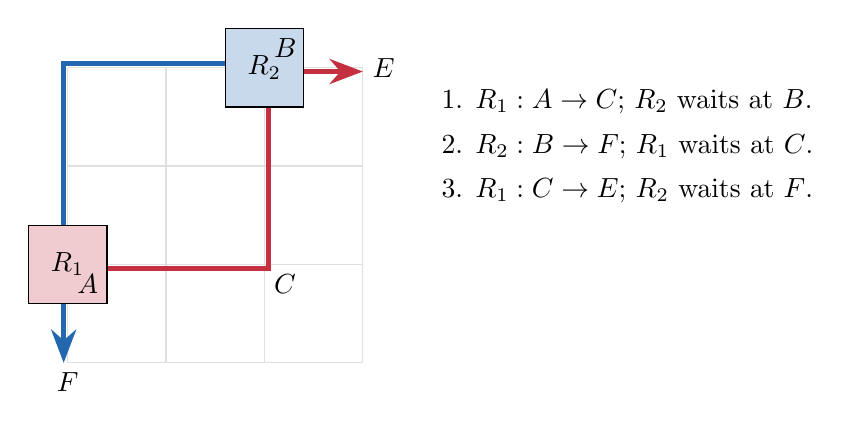
\begin{tikzpicture}[scale=1.25]
\draw[step=1,gray!25] (0,0) grid (3,3);
\draw[rone,line width=2pt,->] (0,0.96)--(2.04,0.96)--(2.04,2.96)--(3,2.96);
\draw[rtwo,line width=2pt,->] (1.96,3.04)--(-.04,3.04)--(-.04,0);
\node[draw,fill=rone!25,minimum width=10mm,minimum height=10mm] at (0,1) {$R_1$};
\node[draw,fill=rtwo!25,minimum width=10mm,minimum height=10mm] at (2,3) {$R_2$};
\node[below right] at (0,1) {$A$};\node[below right] at (2,1) {$C$};
\node[above right] at (2,3) {$B$};\node[right] at (3,3) {$E$};
\node[below] at (0,0) {$F$};
\node[align=left,anchor=west] at (3.7,2.2) {1. $R_1:A\to C$; $R_2$ waits at $B$.\\[4pt]
2. $R_2:B\to F$; $R_1$ waits at $C$.\\[4pt]
3. $R_1:C\to E$; $R_2$ waits at $F$.};
\end{tikzpicture}
\caption{Both routes remain fixed. Partial progress, rather than reversing or
rerouting, resolves the mutual obstruction by the two initial positions.}
\end{figure}

Let progress $u,v\in[0,5]$ count unit grid edges along the respective paths.
Our notation $S_i[a,b]$ denotes the swept region between two progress values;
$S_i[a,a]$ is the footprint at a waiting position. The witness is
\begin{equation}
\begin{split}
S_1[0,2]\cap S_2[0,0]&=\varnothing,\\
S_1[2,2]\cap S_2[0,5]&=\varnothing,\\
S_1[2,5]\cap S_2[5,5]&=\varnothing.
\end{split}\label{eq:witness}
\end{equation}
In contrast, $S_1[0,5]\cap S_2[0,0]\ne\varnothing$ and
$S_2[0,5]\cap S_1[0,0]\ne\varnothing$. Thus neither robot can complete its
\emph{entire} route while the other remains at its start. This is a failure of
whole-route serialization, not proof that action-level dependencies are cyclic.

\clearpage
\section{A coordination-space view: where the choice occurs}
For this square-envelope instance define
\begin{equation}
\mathcal O=\{(u,v): S_1[u,u]\cap S_2[v,v]\ne\varnothing\}.
\end{equation}
Contact counts as interference. In grid units the pairwise coordinate clearance
threshold is $1.5/2=0.75$. The two connected components are
\begin{align}
\mathcal O_A&=[0,0.75]\times[3.25,4.75],\\
\mathcal O_B&=([3.25,4]\times[0,0.75])\ \cup\
 &\qquad\{(u,v):4\le u\le4.75,\ 0\le v\le4.75-u\}.\nonumber
\end{align}
The triangular part of $\mathcal O_B$ results from the two robots moving away
from $B$ in opposite horizontal directions. This diagram uses our squares;
the native Segment Graph paper uses discs and a discrete progress model.

\begin{figure}[h]
\centering
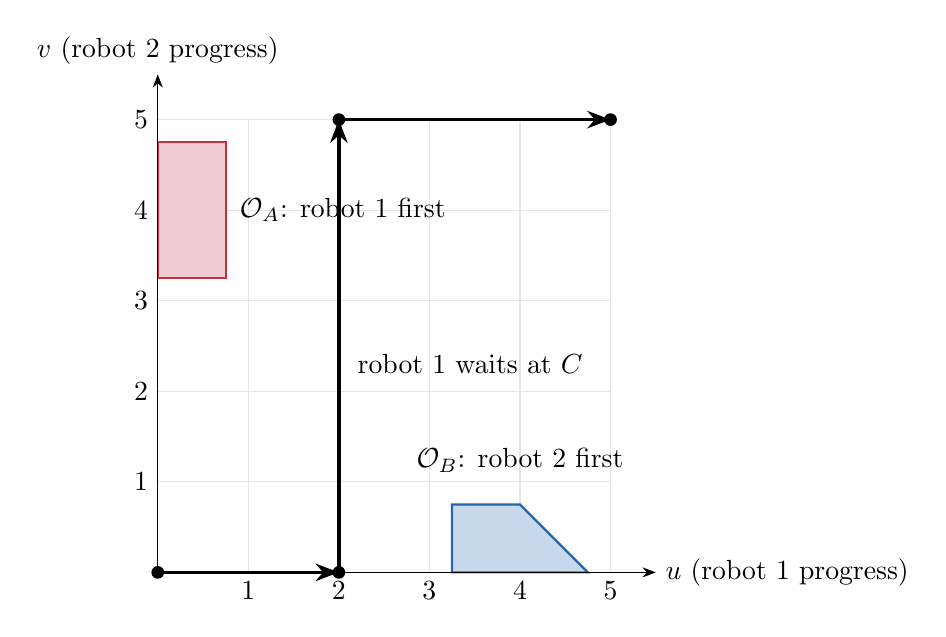
\begin{tikzpicture}[scale=1.15]
\draw[step=1,gray!20] (0,0) grid (5,5);
\fill[rone!25] (0,3.25) rectangle (.75,4.75);
\fill[rtwo!25] (3.25,0)--(4.75,0)--(4,.75)--(3.25,.75)--cycle;
\draw[rone,thick] (0,3.25) rectangle (.75,4.75);
\draw[rtwo,thick] (3.25,0)--(4.75,0)--(4,.75)--(3.25,.75)--cycle;
\draw[->] (0,0)--(5.5,0) node[right] {$u$ (robot 1 progress)};
\draw[->] (0,0)--(0,5.5) node[above] {$v$ (robot 2 progress)};
\foreach \x in {1,...,5} {\node[below] at (\x,0) {\x};\node[left] at (0,\x) {\x};}
\draw[very thick,->] (0,0)--(2,0);
\draw[very thick,->] (2,0)--(2,5);
\draw[very thick,->] (2,5)--(5,5);
\foreach \p in {(0,0),(2,0),(2,5),(5,5)} \fill \p circle(2pt);
\node[right] at (.8,4) {$\mathcal O_A$: robot 1 first};
\node[above] at (4,1) {$\mathcal O_B$: robot 2 first};
\node[right] at (2.1,2.3) {robot 1 waits at $C$};
\end{tikzpicture}
\caption{The monotone path $(0,0)\to(2,0)\to(2,5)\to(5,5)$ is the three-stage
witness. There are two different local passage orders, not one global robot priority.}
\end{figure}

The obstacle near $A$ must be passed with robot 1 clearing $A$ before robot 2
arrives. Near $B$, robot 2 must clear $B$ before robot 1 arrives. A graph with
only two whole-route vertices collapses these different interactions into
$R_1\to R_2\to R_1$. That quotient loses the positions of the constraints along
the routes. It is not the action or segment graph used by the cited methods.

\clearpage
\section{ADG: an explicit compilation of the example}
Name the five translation actions of robot 1 $a_1,\ldots,a_5$ and those of
robot 2 $b_1,\ldots,b_5$. Let $s(x),g(x),t(x)$ be an action's source,
destination and nominal starting rank. Choose the valid nominal serialization
\begin{equation}
(a_1,a_2,b_1,b_2,b_3,b_4,b_5,a_3,a_4,a_5).
\label{eq:rank}
\end{equation}
Ranks are $0,\ldots,9$ in this list, not physical motion durations. Each action
may be allotted enough actual time to finish. In-place rotations can be inserted
as additional own-robot actions; they are omitted from this translational
compilation. This is not a complete reproduction of the warehouse robot model.

ADG Algorithm 1 adds own-robot sequence edges and Type 2 edges satisfying
\begin{equation}
s(x)=g(y),\quad t(x)\le t(y),\quad \operatorname{robot}(x)\ne\operatorname{robot}(y)
\quad\Longrightarrow\quad x\to y.\label{eq:adg}
\end{equation}
For these ten actions its inter-robot output is exactly
\begin{equation}
E_{\rm inter}^{\rm ADG}=\{a_1\to b_4,\ b_1\to a_4\}.
\end{equation}
The first edge says robot 1 must leave $A$ before robot 2 moves into $A$.
The second says robot 2 must leave $B$ before robot 1 moves into $B$.

\begin{figure}[h]
\centering
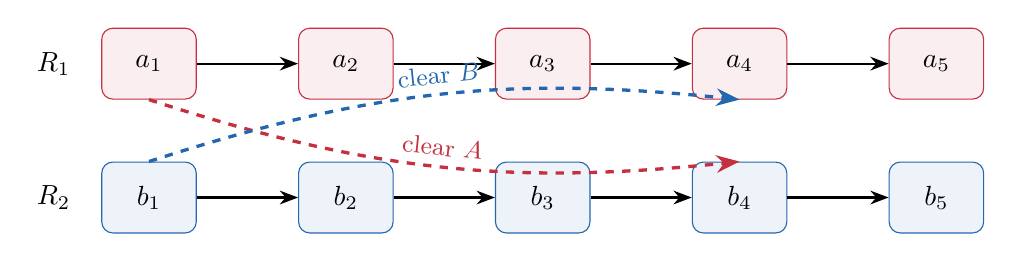
\begin{tikzpicture}[x=2.5cm,y=1.7cm]
\foreach \k in {1,...,5} {
 \node[act,draw=rone,fill=rone!8] (a\k) at (\k,1) {$a_\k$};
 \node[act,draw=rtwo,fill=rtwo!8] (b\k) at (\k,0) {$b_\k$};}
\foreach \k/\l in {1/2,2/3,3/4,4/5} {\draw[seq] (a\k)--(a\l);\draw[seq] (b\k)--(b\l);}
\draw[dep,rone] (a1.south) to[bend right=12] node[above,sloped,font=\small] {clear $A$} (b4.north);
\draw[dep,rtwo] (b1.north) to[bend left=12] node[above,sloped,font=\small] {clear $B$} (a4.south);
\node[left] at (.65,1) {$R_1$};\node[left] at (.65,0) {$R_2$};
\end{tikzpicture}
\caption{The compiled action graph is acyclic. Dashed edges are inter-robot
constraints; horizontal arrows preserve each robot's own path order.}
\end{figure}

Equation~\eqref{eq:rank} is a topological ordering and executes our witness.
The graph does not require exactly those three stages: it also permits safe
interleavings and potentially greater concurrency. A robot's next action is
released when its relevant predecessors finish, not when the other robot's whole
path finishes. This is the point of the ADG execution rule [1, Sec.~IV-B].

\textbf{What has and has not been established.} This example is representable
by ADG; it is not a counterexample to ADG. Its construction takes a valid nominal
plan as input. Providing the plan above proves representability, but does not
show that Algorithm 1 alone discovers the passage orders from two bare paths.

\clearpage
\section{Segment Graph: the local orders are also representable}
The Segment Graph [2] assigns a passage label to each connected coordination
obstacle, rather than a single priority to an entire robot. For this example
the labels are $\ell(\mathcal O_A)=1$ and $\ell(\mathcal O_B)=2$.
At the event-segment level the graph has the following form:
\begin{figure}[h]
\centering
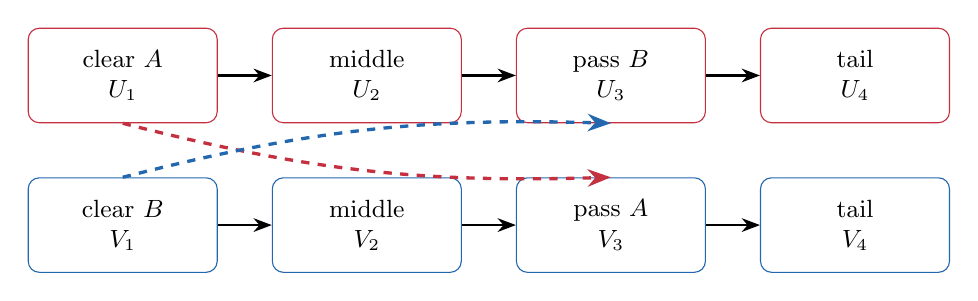
\begin{tikzpicture}[x=3.1cm,y=1.9cm,
seg/.style={draw,rounded corners,align=center,minimum width=24mm,minimum height=12mm,font=\small}]
\node[seg,draw=rone] (u1) at (0,1) {clear $A$\\$U_1$};
\node[seg,draw=rone] (u2) at (1,1) {middle\\$U_2$};
\node[seg,draw=rone] (u3) at (2,1) {pass $B$\\$U_3$};
\node[seg,draw=rone] (u4) at (3,1) {tail\\$U_4$};
\node[seg,draw=rtwo] (v1) at (0,0) {clear $B$\\$V_1$};
\node[seg,draw=rtwo] (v2) at (1,0) {middle\\$V_2$};
\node[seg,draw=rtwo] (v3) at (2,0) {pass $A$\\$V_3$};
\node[seg,draw=rtwo] (v4) at (3,0) {tail\\$V_4$};
\foreach \p/\q in {u1/u2,u2/u3,u3/u4,v1/v2,v2/v3,v3/v4} \draw[seq] (\p)--(\q);
\draw[dep,rone] (u1.south) to[bend right=8] (v3.north);
\draw[dep,rtwo] (v1.north) to[bend left=8] (u3.south);
\end{tikzpicture}
\caption{Local obstacle-label edges $U_1\to V_3$ and $V_1\to U_3$ are compatible.
This is an event-segment mapping; the paper's native model is discrete and disc-shaped.}
\end{figure}

\textbf{A concrete native-model realization.} To avoid pretending that squares
and discs are identical, take discs of radius $r=0.76$ m and sample each $2$ m
route edge every $0.5$ m. Use zero-based progress indices $k,l\in\{0,\ldots,20\}$
(the paper uses one-based indices). Its native test
$\|\pi_1(k)-\pi_2(l)\|<2r$ yields two connected obstacle components.
The first has projections $k=0{:}3$, $l=13{:}19$; the second has projections
$k=13{:}19$, $l=0{:}3$. Accordingly, the four vertex ranges for either route
are $0{:}3$, $4{:}12$, $13{:}19$, and the final index $20$.
Reading these as entry/clearance event segments gives the diagram above by
Definition 3: the last segment overlapping an obstacle precedes the other
robot's first segment overlapping it. The two components' detailed shapes differ
from the square-envelope diagram, but their incidence and selected passage
orders agree. This disc instance is a comparison model, not our RMFS geometry.

\textbf{The essential qualification.} Segment Graph Definition 4 requires every
robot's path to avoid the other robots' start and goal positions. Our example
violates the start condition twice: $A\in P_2$ and $B\in P_1$.
Therefore its Theorem 1's implication from deadlock to an active graph cycle
cannot be applied to this instance merely because the graph is acyclic.
Nevertheless, the explicit witness completes the paths and the labeled graph
can express its orders. \emph{Being outside a theorem's assumptions is not the
same as being beyond the method's representational ability.}

The paper's nominal jointly feasible trajectories already supply the obstacle
labels. Online label repair does not itself establish complete search over all
labels for arbitrary initially uncoordinated paths.

\clearpage
\section{SCALE: exact action-sweep conflicts for this instance}
Use the same ten translation actions, square envelope, and ranks in
Equation~\eqref{eq:rank}. Direct rectangle-union intersection gives exactly four
inter-robot conflicting action pairs:
\begin{equation}
\mathcal C=\{(a_1,b_4),(a_1,b_5),(a_4,b_1),(a_5,b_1)\}.
\end{equation}
Applying SCALE's HAPG Definition III.1 and Algorithm 1 [4] therefore yields
\begin{equation}
E_{\rm inter}^{\rm HAPG}=\{a_1\to b_4,\ a_1\to b_5,\ b_1\to a_4,\ b_1\to a_5\}.
\end{equation}
Two edges are transitively redundant: $a_1\to b_5$ follows through $b_4$,
and $b_1\to a_5$ follows through $a_4$. The transitive reduction is exactly
the displayed ADG. Thus SCALE's more geometric conflict predicate does not
prevent it from representing our alternating-progress witness.

\textbf{Capsule interpretation.} Conflicts at $A$ pair $a_1$ with the consecutive
span $(b_4,b_5)$; conflicts at $B$ pair $b_1$ with $(a_4,a_5)$.
These are the spans suggested by the conflict signatures. No MILP switch or
capsule reordering is needed to execute the supplied ranks. This does not test
SCALE's capsule extraction or optimization implementation, nor show that either
order is reversibly selectable from the initial state. In particular, an
initially occupied waiting footprint must not be erased when reasoning about
alternative orders. SCALE's guarantee assumes a feasible rank-consistent input.

\section{SADG and the input-plan distinction}
SADG [3] likewise begins with a valid MAPF solution and constructs a spatially
exclusive action graph. Consecutive grid positions here are $2$ m apart, so the
$1.5$ m squares at those positions are spatially exclusive. With one translation
per graph vertex and the supplied nominal order, its Algorithm 1 produces the
same two inter-robot edges as the ADG above. In-place rotations may be grouped
with a translation by its spatial-exclusivity rule.
An initially acyclic graph therefore represents this witness without requiring
an online order switch. That is a compilation statement; it is not a run of
SADG's optimizer. Its recursive-feasibility results concern permissible updates
of an already valid execution graph, not an unconditional solver for arbitrary
fixed spatial paths.

\begin{center}\small
\begin{tabular}{p{23mm}p{44mm}p{76mm}}
\toprule
Method & This example's graph & What this comparison establishes\\
\midrule
ADG & Two inter-robot edges; DAG & Witness represented from a valid nominal plan.\\
Segment Graph & Two local label edges; DAG & Orders representable; start-avoidance theorem assumption fails.\\
SADG & Same two edges in the stated compilation & Valid initial SE-ADG available; optimizer not evaluated.\\
SCALE HAPG & Four edges; same transitive reduction & Geometric conflicts and witness represented; planner/MILP not executed.\\
\bottomrule
\end{tabular}
\end{center}

\clearpage
\section{Verdict and what is still worth investigating}
\textbf{Verdict: the alternating-progress example is not evidence of a missing
capability in existing action/segment dependency representations.} The apparent
cycle exists only after collapsing different portions of each path into one
robot-level vertex. Preserving those portions yields an acyclic execution graph.

This corrects a possible overstatement in our earlier discussions: mutual
whole-route obstruction does not imply an action-level cycle that must somehow
be executed. Our three-stage solution can be compiled into existing graph
representations. It should eventually be included in our paper as an explanatory
example, but not presented as a new capability without a stronger comparison.

\begin{enumerate}
\item \textbf{Representation is already available.} Action-level and local
obstacle-level orders can encode the witness. Different conflicts between the
same two robots may have different passage orders.
\item \textbf{Construction remains a separate question.} ADG, SADG and the HAPG
compilation consume a valid ordered plan. Segment Graph consumes nominal
coordinated trajectories. To compare our solver, one must also compare the
planners or order-search procedures supplying those inputs. SCALE includes a
planning module, so absence of search in its graph compiler is not absence of
search from the complete system.
\item \textbf{Endpoint handling deserves a precise comparison.} Our instance is
outside Segment Graph Definition 4. That is a theorem-scope difference worth
documenting, not yet a new theorem or a demonstrated algorithmic advantage.
\item \textbf{No new sufficiency claim is made here.} The three disjoint sweep
pairs in Equation~\eqref{eq:witness} certify this particular completion. Extending
our general sufficient condition is deliberately postponed.
\end{enumerate}

\paragraph{Verification record.}
The path coordinates were read from the existing example. Our existing exact
rectangle-union sweep backend checked all three witness stages, all $25$
inter-robot translation-action pairs and the resulting four conflicts. The ADG
source/destination rule was enumerated for all ordered inter-robot pairs and
gave the two stated edges. Topological ordering~\eqref{eq:rank} was checked for
both action graphs. The native disc comparison was enumerated over all
$21^2$ sampled position pairs to check its two components and projections.
These are finite analytical checks, not a DEVS run, a runtime comparison, or
execution of any authors' implementation.

\begin{thebibliography}{9}\small
\bibitem{adg} W. H\"onig et al., ``Persistent and Robust Execution of MAPF
Schedules in Warehouses,'' RA-L, 2019, Sec.~IV-B and Algorithm 1.
\url{https://whoenig.github.io/publications/2019_RA-L_Hoenig.pdf}.
\bibitem{sg} A. Coskun, J. M. O'Kane, and M. Valtorta, ``Deadlock-Free Online
Plan Repair in Multi-robot Coordination with Disturbances,'' FLAIRS, 2021,
Definitions 2--4, Theorem 1 and Figure 4.
\url{https://jokane.net/pubs/CosOKaVal21.pdf}.
\bibitem{sadg} A. Berndt et al., ``Receding Horizon Re-Ordering of Multi-Agent
Execution Schedules,'' TRO, 40, 1356--1372, 2024, Algorithm 1 and Assumption 2.
\url{https://doi.org/10.1109/TRO.2023.3344051}.
\bibitem{scale} B. Cao, ``From Real-Time Planning to Reliable Execution:
Scalable Coordination for Heterogeneous Multi-Robot Fleets in Industrial
Environments,'' arXiv:2607.00591v2, 2026, Definition III.1, Algorithm 1,
Lemma III.2 and Sec.~IV-B.
\url{https://arxiv.org/abs/2607.00591v2}.
\end{thebibliography}
\end{document}
